\documentclass{standalone}

\usepackage{tikz}
\usepackage{amsmath}
\usetikzlibrary{arrows}


\begin{document}
\begin{tikzpicture}[>=latex]
	% Ebene
	%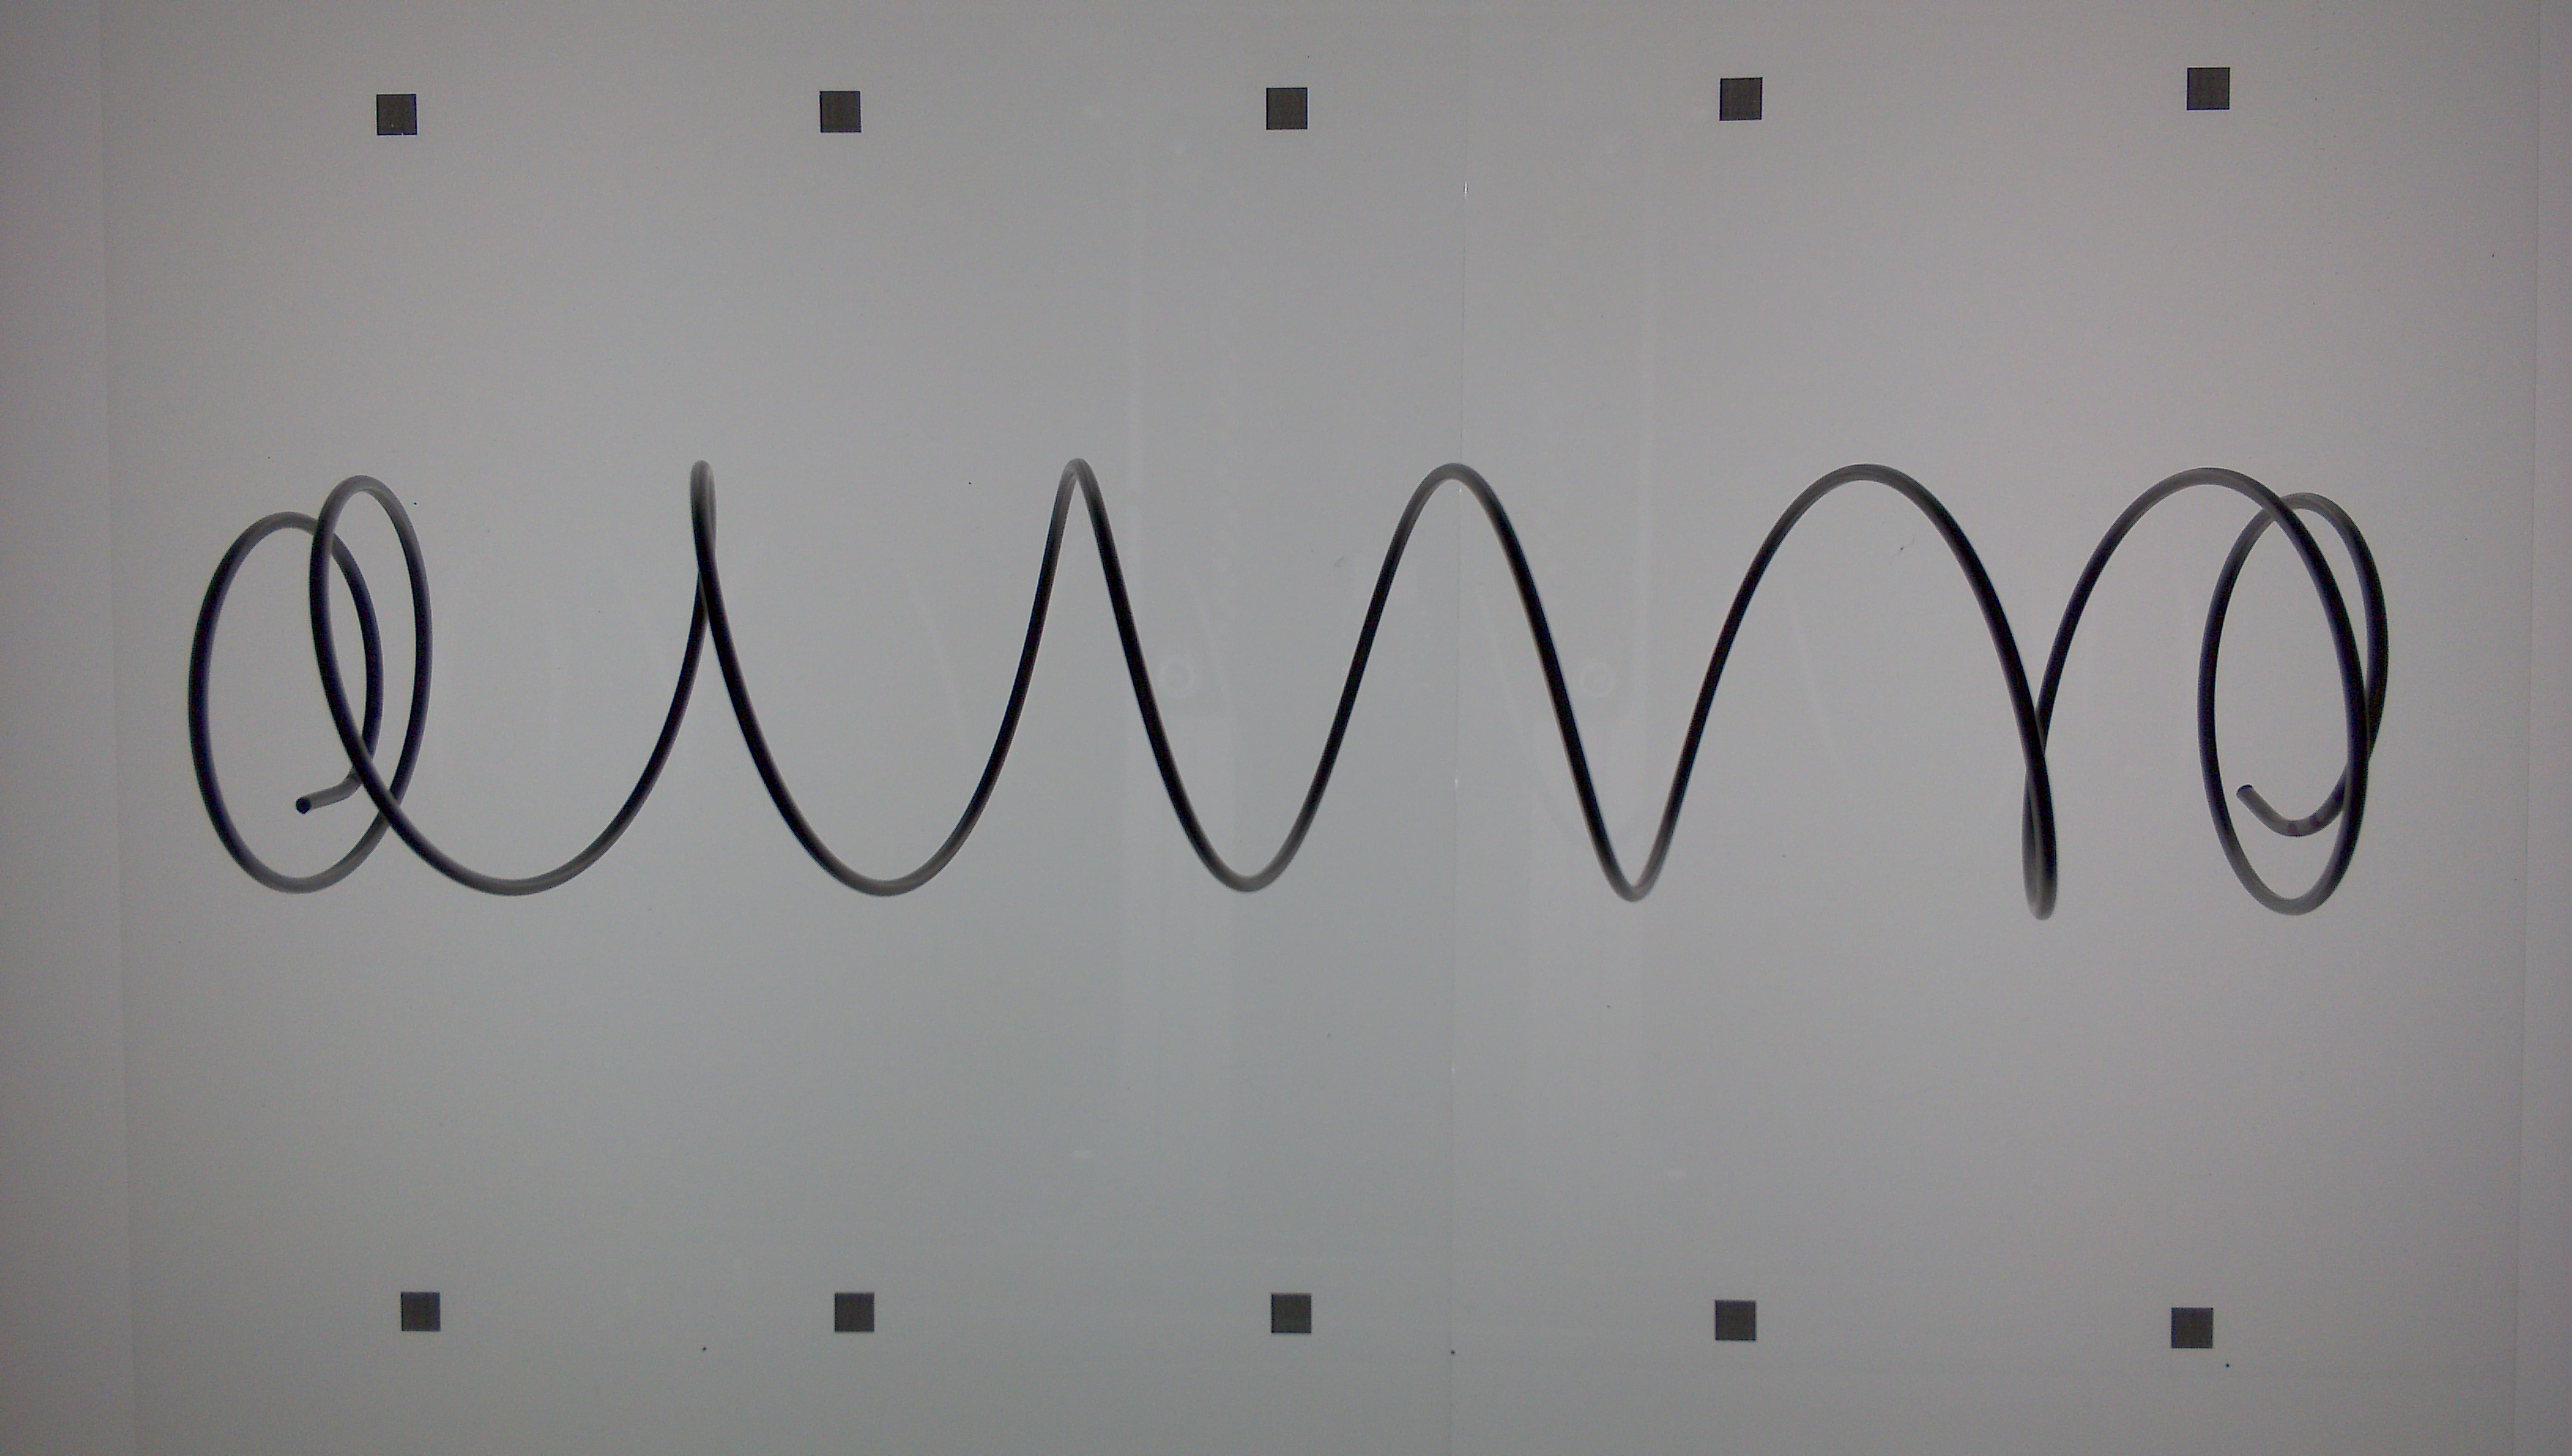
\includegraphics[width=150pt]{bim1.png} at (0,0);

	\node[inner sep=0pt] (russell) at (0,0)
	{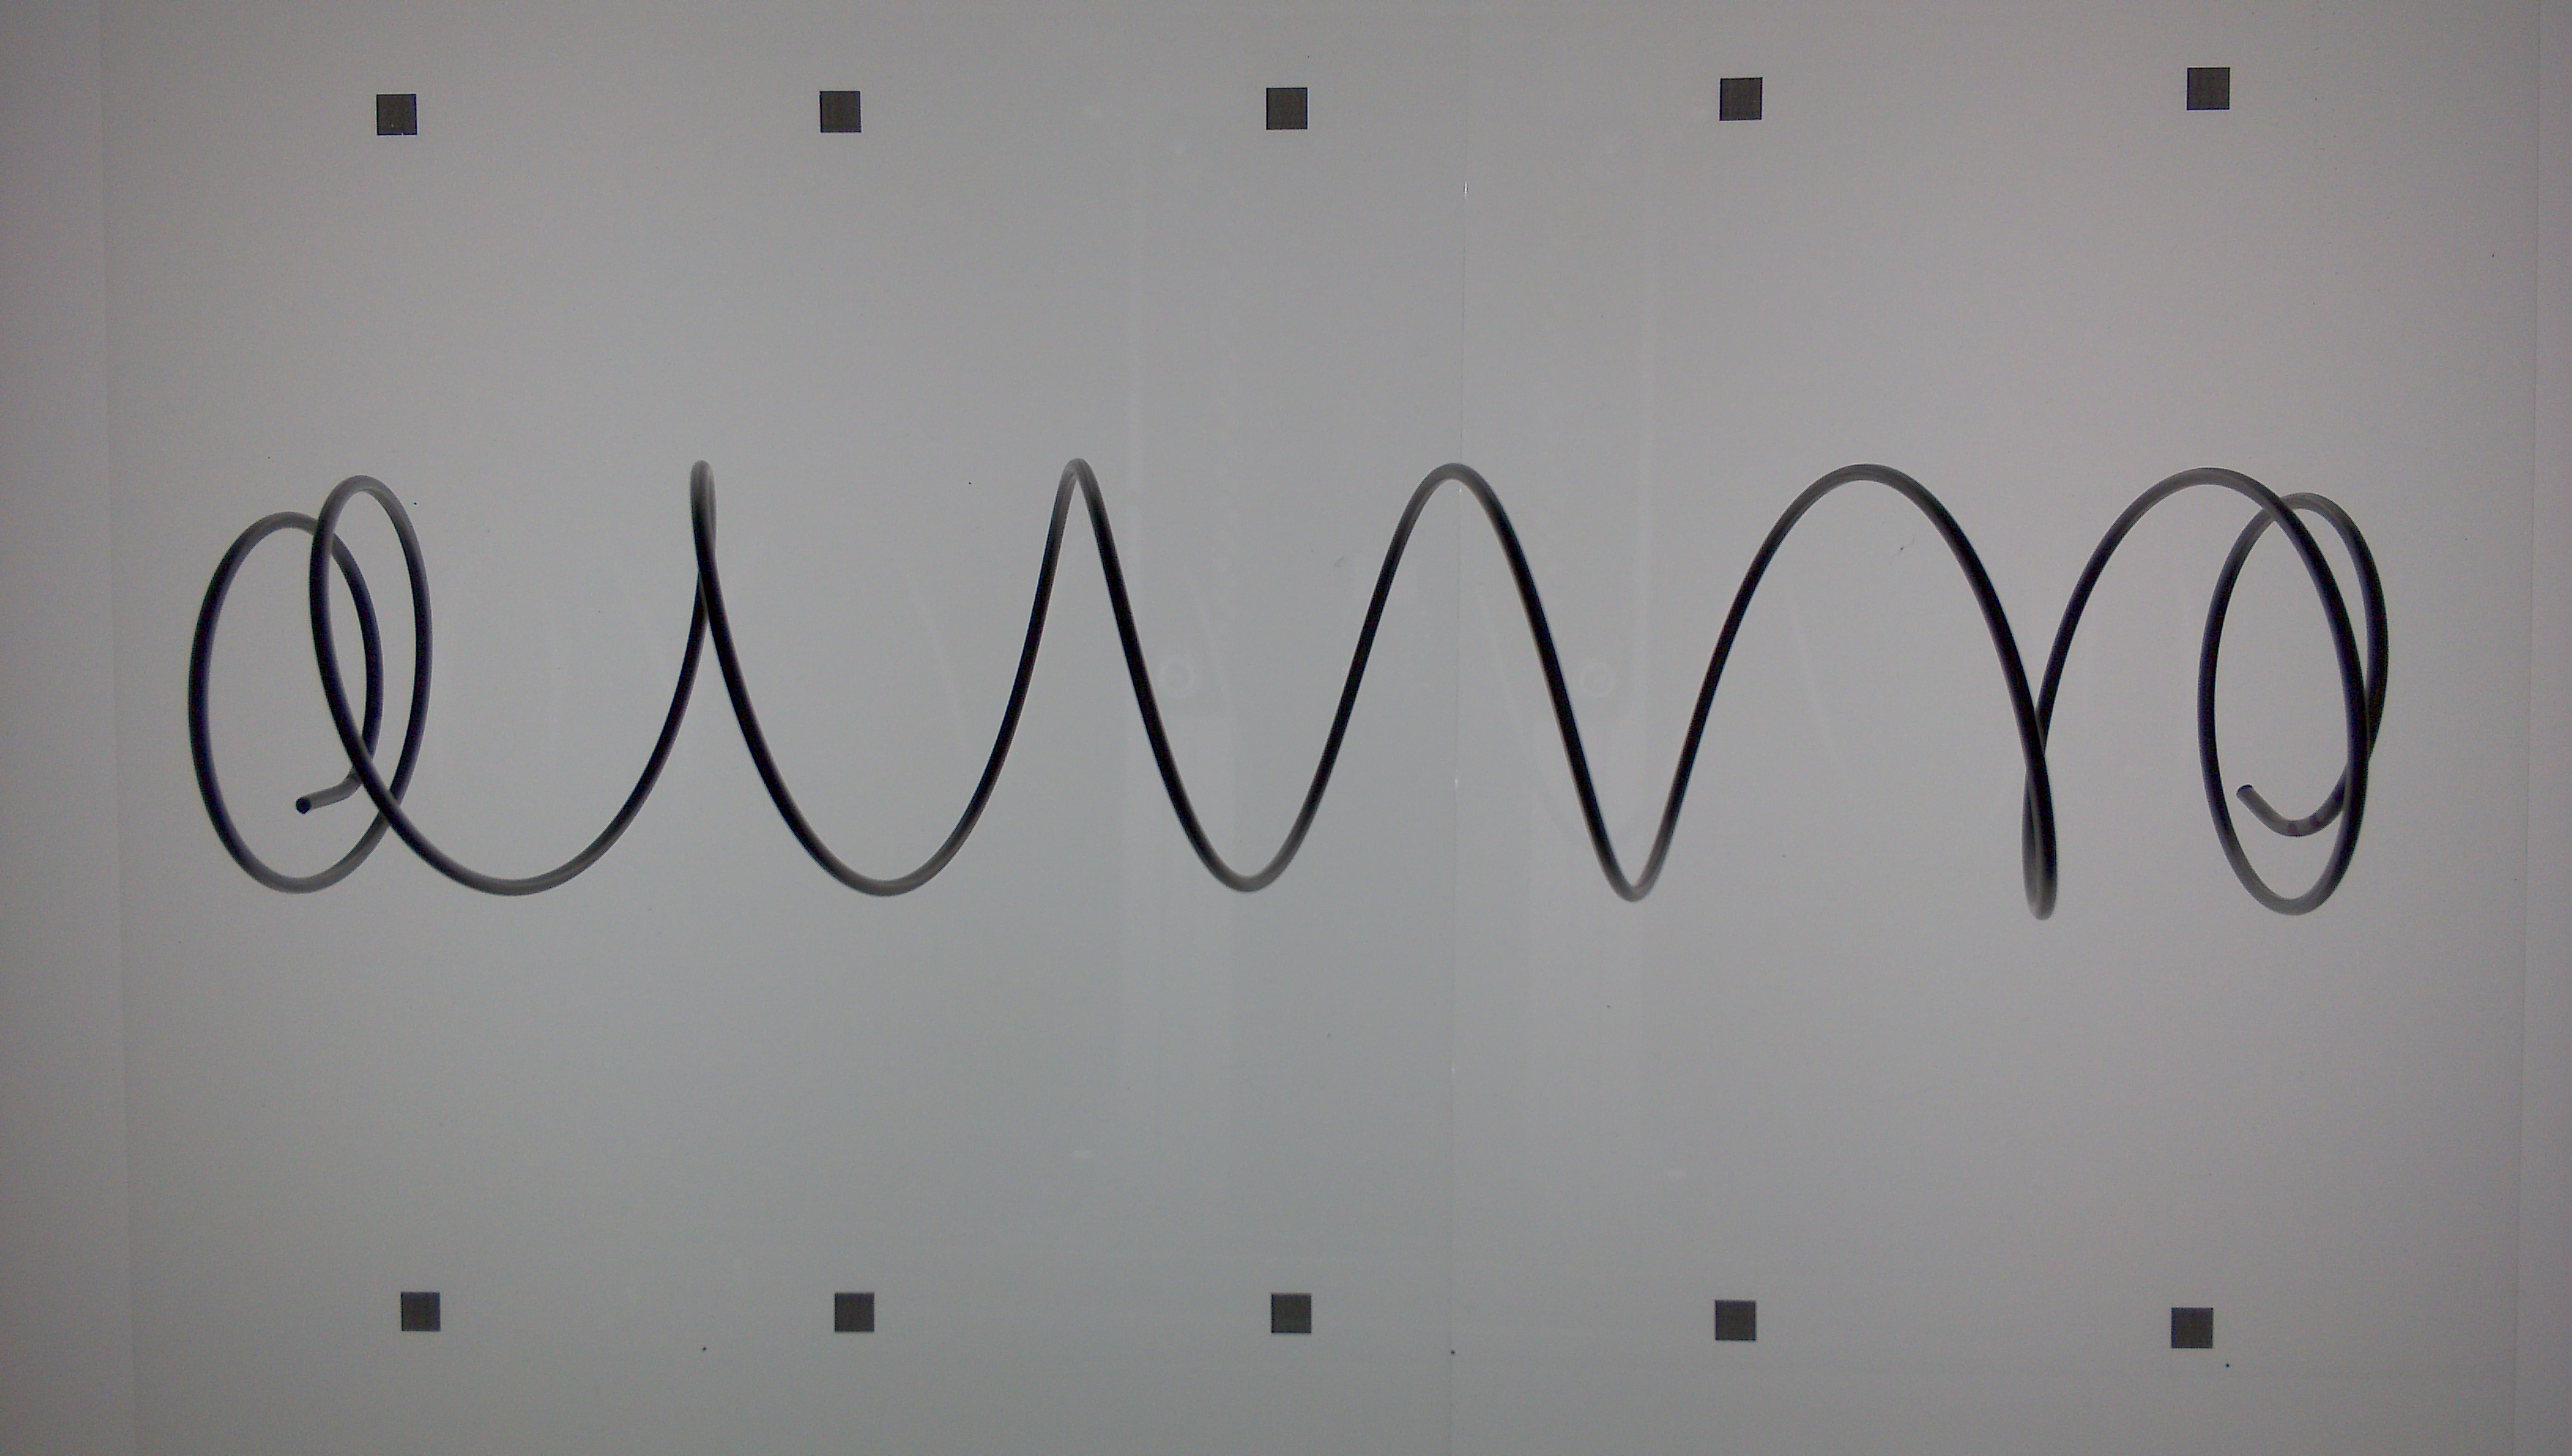
\includegraphics[width=10cm, height=6cm]{bim1.png}};
	\draw[color = black!30!white , dashed, thick] (-5,-2)--(5,-2);
	\draw[color = red, line width=0.5mm ] (-4.97,-2)--(-4.97,2);
	\draw[color = red ] (-4.8,1.5)node [color=red,right]{First trigger line}-- (-5,1);
	\draw[color = black!30!white , dashed, thick] (-5,2)--(5,2);

	\draw[color = blue, line width=0.5mm ] (0-5/3,-2)--(0-5/3,2);
	\draw[color = blue ] (-1.5,1.5)node [ color=blue,right]{Second trigger line}-- (0-5/3,1);
	\draw[color = blue, line width=0.5mm ] (0+5/3,-2)--(0+5/3,2);
	\draw[color = blue ] (1.8,1.5)node [ color=blue,right]{Third trigger line}-- (0+5/3,1);
	
	\draw[color = blue ] (4.8,-1.5)node [ color=blue,left]{Fourth trigger line}-- (5,-1);
	\draw[color = blue, line width=0.5mm ] (4.97,-2)--(4.97,2);
	\draw[<->,color = black!10!white](-0.5,3)-- node[left]{sep}(-0.5,2);
	\draw[<->,color = black!10!white](-0.5,-3)-- node[left]{sep}(-0.5,-2);
	
	\end{tikzpicture}
\end{document}	